	
\subsection{Information and the Checkerboard}
	We begin by developing two fundamental measures of information theory, the entropy of one random variable and the mutual information of two. Let $X$ be a spatial variable, such as a set of coordinates in space or a neighborhood name. Let $Y$ be a compositional variable that we aim to study, defined on an alphabet $\mathcal{Y}$. In the simple case in which $\mathcal{Y}  = \{\text{Black, White}\}$, Figure \ref{fig:toy} illustrates a range of possible joint distributions $p(X,Y)$. Comparing the completely undiverse city (a) and the spatially uniformly diverse (b) motivates the first fundamental information measure, the entropy:
	\begin{equation}
		H(Y) \triangleq -\E_Y[\log p(Y)] = - \sum_{y \in \mathcal{Y}} p(y) \log p(y)\;.
	\end{equation}
	The entropy measures how evenly the global marginal distribution $p(Y)$ is distributed over the alphabet $\mathcal{Y}$. Epistemically, $H(Y)$ measures the difficulty in guessing the random variable $Y$, given no further information. $H(Y) = 0$ when $Y$ always takes a single value, such as in city (a) -- perfect guessing is possible. On the other hand, $H(Y)$ achieves its maximum of $H(Y) = \log \abs{\mathcal{Y}}$ when $Y$ is uniformly distributed on $\mathcal{Y}$, as in city (b). The entropy $H(Y)$ is this sufficient to distinguish the presence of global diversity from its absence. On the other hand, the entropy $H$ is unable to distinguish between the spatial uniformity of (b) and the spatially variability of (c). To distinguish these two cities we may use the mutual information, which is defined in terms of the Kullback-Leibler divergence $D$:
	\begin{align}
		D[p(Z)\|q(Z)] &\triangleq \sum_z p(z) \log \frac{p(z)}{q(z)} \\
		I(X,Y) &\triangleq D[p(X,Y) \| p(X)p(Y)] = \E_X[D[p(Y|X)\|p(Y)]]
	\end{align}
	Though not a true metric, the divergence $D$ is interpretable a measure of distance in the space of probability distributions, and so $I(X,Y)$ may be interpreted as the distance between the true joint distribution $p(X,Y)$ and the product of marginals $p(X)p(Y)$. Since the latter expresses statistical independence between $X$ and $Y$, $I(X,Y)$ measures the extent to which $X$ and $Y$ are dependent. Epistemically, $I(X,Y)$ measures the extent to which knowledge of $X$increases possible accuracy in guessing $Y$. In city (b), $X$ and $Y$ are independent: knowing $X$ (where an individual lives) conveys no information about that $Y$ (that individual's race).  In city (c), on the other hand $X$ and $Y$ are completely dependent: if you know where someone lives, you know their race with 100\% confidence, and $I(X,Y)$ achieves its maximum. 

	City (d) shares with city (c) the fact that race is completely determined by residence. However, city (d) embodies the ``checkerboard problem'': measures that use only the joint distribution $p(X,Y)$ without additionally considering the spatial information contained within $X$ will evaluate city (d) to be the same as city (c), despite their considerably different patterns of racial separation and potentially very different implications for planning and policy. A recent working paper \cite{Roberto2015} provides one highly operational approach to this problem, using road network topology and a weighting function that decays with distance to define a localized measure based on the Kullback-Leibler divergence. Here we pursue an alternative strategy, showing that a localization of the mutual information both measures spatial variation in race and corresponds to the estimation of a fundamental statistical property of the distribution $p(X,Y)$. 

	\begin{figure}
		\centering
		  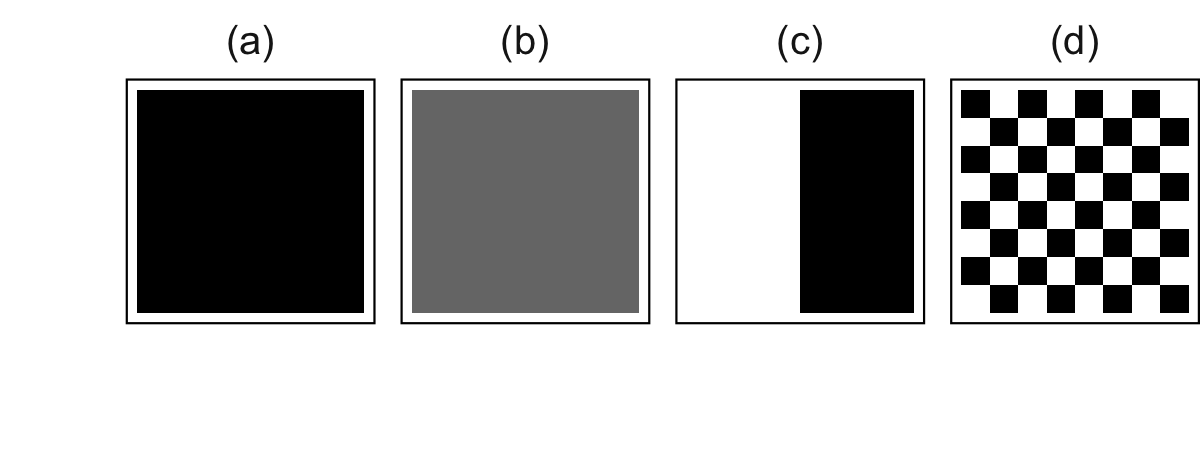
\includegraphics[width=.7\linewidth]{figs/checkerboard.png}
		\centering
		  \begin{tabular}{c | c c c}
			  City & $H(Y)$ & $I(X,Y)$ & $J(X,Y)$ \\
			  \hline			
			  (a) & 0.0 & 0.0 & 0.0\\
			  (b) & 0.7 & 0.0 & 0.0\\
			  (c) & 0.7 & 0.7 & 0.6\\
			  (d) & 0.7 & 0.7 & 2.7\\
			  \hline  
			\end{tabular}
		\caption{Information theory and the checkboard problem: model cities with various kinds of spatial diversity can be distinguished through progressively more subtle spatial information measures.}
		\label{fig:toy}
		\end{figure}

\subsection{Measuring Socio-Spatial Complexity}

	We will now derive a measure that solves the ``checkerboard problem'' by distinguishing the toy cities (c) and (d). To motivate our methods, we  consider an idealized scenario in which we have a differentiable field $p(y|x)$ of observed probability distributions for each $x \in M \subset \R^n$, where the metric space $M$ is interpretable as the ``map'' on which we work. 

	Fix a point $x_0 \in M$ and a radius $r > 0$. Let $B_r(x_0)$ denote the ball of radius $r$ about $x_0$. Then, define the \emph{local mutual information in radius $r$} as the mutual information between $X$ and $Y$, restricted to the small ball $B_r(x_0)$ about $x_0$:
	\begin{equation}
		I_r(x_0) \triangleq \E_X[D[p(\cdot|X)\| p(\cdot|X \in B_r(x_0))]|X \in B_r(x_0)] \label{eq:local}
	\end{equation}
	Intuitively, $I_r(x_0)$ measures how much knowing the ``location'' $x$ adds to our information about the category $Y$, or, equivalently, how much the probability field $p(y|x)$ varies with $x$ in a small neighborhood of $x_0$. It is therefore a natural measure of local complexity, aligned in approach with the global mutual information but designed to detect local variation. As expected, $I_r(x_0) = 0$ if and only if $p(y|x)$ is constant for each $y$ in the ball $B_r(x_0)$; that is, if within $B_r(x_0)$ the field $p(y|x)$ resembles toy city (b) in Figure \ref{fig:toy}. In the definition \eqref{eq:local}, $r$ may be thought of as the spatial resolution at which we conduct analysis, and $I_r(x_0)$ is highly dependent on $r$. However, it is possible to show that $I_r(x_0)$ is related to a fundamental statistical property of the probability field $p(y|x)$ that is resolution-independent. Under the stated conditions, the following approximation holds: 

	\begin{equation}
		\frac{I_r(x)}{r^2} \cong \frac{1}{4} \text{trace } J_Y(x)\;, \label{eq:approx}
	\end{equation}
	where $J_Y(x)$ is the Fisher information matrix in $Y$ about $x$, defined as 
	\begin{equation}
		J_Y(x) \triangleq \E_Y\left[ (\nabla_x \log p(Y|x))(\nabla_x \log p(Y|x))^T \right]\;.
	\end{equation}
	A formal statement and proof of \eqref{eq:approx} are provided in Appendix 2. The Fisher information $J_Y$ is a fundamental quantity in statistics and information theory. From a geometric perspective, $J_Y$ provides the natural intrinsic metric in the geometric space of probability distributions parameterized by the spatial variable $x$. Equation \eqref{eq:approx} therefore expresses a relationship between the local mutual information $I_r(x)$ and the information geometry of the underlying probability field. Corresponding to the fact that $I_r(x_0)$ vanishes if and only if $p(y|x)$ is constant in $B_r(x_0)$, $J_Y(x_0) = 0$ if and only if $\nabla_x p(y|x_0) = 0$ for all $y$. This implies that $x_0$ is a stationary point, about which the probability field $p(y|x_0)$ exhibits only small (2nd order or smaller) changes with respect to changes in $x$. 

	Since the Fisher information is a strictly local measure of statistical variability around $x$, we can aggregate the Fisher information to derive a measure of average local variability. The \emph{mean local information} is 
	\begin{equation}
	J(X,Y) \triangleq \E_X[\text{trace }J_Y(X)] \label{eq:def_J}
	\end{equation} 
	As demonstrated in Figure \ref{fig:toy}, $J(X,Y)$ distinguishes cities (c) and (d), thereby addressing the ``checkerboard problem'' head on. We propose the aggregate quantity $J(X,Y)$ as a third  measure--alongside the entropy $H(Y)$ and mutual information $I(X,Y)$-- as a tool for the information-theoretic structure of spatial compositional complexity. 

	We note that, since 
	\begin{align}
		\text{trace } J_Y(x) &=  \sum_i \E_Y\left[ \left(\frac{1}{p(Y|x)} \frac{\partial p(Y|x)}{\partial x_i}\right)\right]^2\;
	\end{align}
	may be viewed as a weighted norm of the gradient $\nabla_x p(Y|x)$, the quantity 
	\begin{align}
		J(X,Y) &= \E_X[\text{trace } J_Y(X)] \\
		&= \int_M \text{trace } J_Y(X) d\prob_X
	\end{align}
	may be viewed as a cousin to total variation measures often encountered in analysis. 

	The application of this methodology to a discrete data set is conceptually simple. For a given set of tracts, overlay an evenly spaced grid of radius $r$, and measure the mutual information $I_r(x)$ in each grid cell. Then, when data and grid resolutions are sufficiently high, $4I_r(x) / r^2$ approximates the quantity $\text{trace }J_Y(x)$, which can then be aggregated across the data set. We provide a more formal statement of this computation in the appendix. 

\subsection{Information Measures and Segregation Studies}

	Considerable attention has been paid to relating segregation indices to intuitive concepts of diversity and segregation. We note here that the mutual information $I(X,Y)$ and mean local information $J(X,Y)$ correspond closely to the two dimensions of segregation formulated in \cite{Reardon2002}. The authors of \cite{Reardon2002} describe \emph{evenness} as ``the extent to which groups are similarly distributed in residential space'' (page 126), and \emph{exposure} as ``the extent that members of one group encounter members of another group...in their local spatial environments.'' The mutual information $I(X,Y)$ may be viewed as a measure of (lack of) evenness, since to say that groups are similarly distributed in residential space is to say that knowing a spatial location conveys little about the race of the people who live there. Large $I(X,Y)$ reflects highly uneven distributions of demographic groups. Complementarily, the mean local information $J(X,Y)$may be viewed as a measure of spatial exposure \emph{for a fixed level of} $I(X,Y)$, as is illustrated by cities (c) and (d) in \ref{fig:toy}. Though distinct, these dimensions are not independent. To see this, note that the most thorough kind of exposure is achieved when $I(X,Y) = J(X,Y) = 0$, as in city (b). Since the concept of exposure only applies in a city with spatial differences, $J(X,Y)$ must be considered jointly with $I(X,Y)$ as a measure of spatial exposure. 

	There has also been much work showing the desirable properties of various segregation indicies. To give a brief sampling, indices should be invariant to changes in overall population size; they should decrease when populations ``even themselves out,'' and they should behave predictably under aggregation. Since we are presenting $I(X,Y)$ and $J(X,Y)$ as a suite of complementary information measures, we consider each in turn. The author of \cite{Roberto2015a} shows that the mutual information $I(X,Y)$ (which she calls the ``Divergence Index'') satisfies these and other desirable properties, generally as well or better than existing alternatives. We highlight one property of $I(X,Y)$ for special note, as this property will be central to our development of natural neighborhood identification. The principle of ``additive decomposability'' \cite{Reardon2002} stipulates that, when the data is grouped along either racial or spatial axes, a good segregation index should split into ``within group'' and ``between group'' components. In the context of the mutual information $I(X,Y)$, additive decomposability is simply the familiar chain rule of mutual information. For concreteness, let $C$ be a random variable giving the cluster label of location $X$; importantly, $C$ is completely determined by $X$. Then, the chain rule expresses additive decomposability as 
	\begin{equation}
		I(X,Y) = I(C,Y) + I(X,Y|C)\;; \label{eq:information_decomp}
	\end{equation}
	i.e. the information I have about $Y$ given that I know $X$ is equal to the information I have if I first learn the cluster $C$, plus the amount of additional information I gain if I subsequently learn the exact location $X$ as well. The first term is interpretable as the between-group information, while the second is interpretable as the within-group information. It is therefore comparable to various ``sum of squares'' decompositions that frequently appear in classical statistics. Indeed, it is possible to show that, when the differences between locations are small, the mutual information can be interpreted as a variance, in which case \eqref{eq:information_decomp} expresses the sum of squares composition directly. A similar version of the chain rule expresses additive decomposability for aggregation of racial groups rather than spatial locations. 

	What of $J(X,Y)$? Below, we provide a brief overview of the properties of $J(X,Y)$. $J(X,Y)$ possesses a variety of intuitive properties, and those that it does not possess either underscore the importance of reading it in conjunction with $I(X,Y)$ or do not apply to explicitly spatial measures.  See \cite{Reardon2002,Reardon2004} for further discussion of these criteria. The mean local information $J(X,Y)$ satisfies: 
	\begin{description}
		\item[Organizational Equivalence:] Both the theoretical definition \eqref{eq:def_J} or the procedure to compute it from tract data remain unchanged when a tract is subdivided into smaller tracts, each of which with identical demographic structure. 
		\item[Size and Density Invariance:] Since $J(X,Y)$ is completely determined by the marginal distribution $p(X,Y)$, it is invariant under changes in population density. 
		\item[Additive Group Decomposability:] When demographic groups are aggregated into super-groups, the chain rule of mutual information applied to the demographic variable $Y$ provides an an additive decomposition of the form $J(X,Y) = J(X,G) + J(X,Y|G)$, which can be interpreted as the sum of a between-groups term and a within-groups term as needed.   
		\item[Scale Interpretability:] We have $J(X,Y) = 0$ if and only if $p(Y|X)$ is constant on each connect component of the metric space $M$. When only one connected component exists, this implies that every locale has the same demographic structure as the global environment. When multiple connected components exist (e.g. the city is divided by a river), demographics must be constant in space on each side of the division. $J(X,Y)$ does not satisfy the additional condition of achieving its maximum value when all locales are monoracial, but this point only emphasizes that $J(X,Y)$ and $I(X,Y)$ should be read jointly. When all locales are monoracial, $I(X,Y)$ achieves its maximum value and $J(X,Y) = 0$. 
		\item[Boundary Independent:] $J(X,Y)$ is defined in terms of a continuous underlying probability distribution $p(X,Y)$, rather than arbitrarily-defined tracts. In computational practice, $J(X,Y)$ is indeed sensitive to the boundaries supplied with the data; however, \eqref{eq:approx} guarantees that this sensitivity vanishes as the resolution grows sufficiently small.  
		\item[Exchanges:] Exchanges that tend to ``smooth out'' demographic distributions in space reduce both $I(X,Y)$ and $J(X,Y)$.  
	\end{description}
	The mean local information $J(X,Y)$ fails to one of the criteria enumerated in \cite{Reardon2002,Reardon2004}; that of \textbf{additive spatial decomposability}. This criterion states that ``If X spatial subareas are aggregated into Y larger spatial areas, then a segregation measure should be decomposable into a sum of within- and between-area components'' \cite{Reardon2004}, page 136. However, considering that we have imposed additional spatial structure on our model, this criterion does not appear to be motivated. Consider, for example, Figure \ref{fig:decomposability}. Aggregating the two central regions transforms (e) into (f), erasing all spatial variability. Any measure should therefore have a between-groups component equal to 0. On the other hand, the within-groups component can only consider the middle white/black boundary between the central two regions. The sum of the between-groups and within-groups components must therefore consist only in information included in the middle boundary. However, the spatial variability in city (e) is not exhausted by this middle boundary; there are a total of six other frontiers of racial difference that should be considered in any spatial segregation measure. We therefore content that additive decomposability is a desideratum of nonspatial measures (it is satisfied by $I(X,Y)$), but not of explicitly spatial ones. 
	\begin{figure}
		\centering
		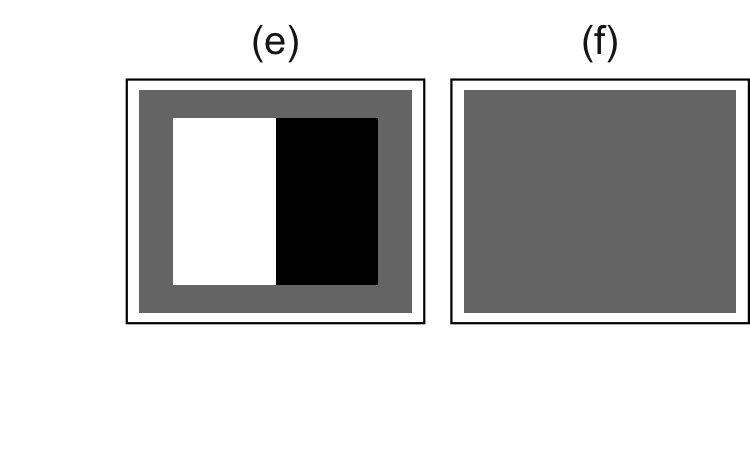
\includegraphics[width=.5\textwidth]{figs/decomposability.png}
		\caption{A problem with additive spatial decomposability: aggregating the inner two regions transforms (e) into (f), smoothing out all spatial variability. A ``between groups'' term must therefore vanish, while a ``within-groups'' term considers only the inner boundary; not the outer ones.}
		\label{fig:decomposability}
	\end{figure}
	We have not exhausted the full complement of desiderata for segregation measures. However, many of the remaining ones -- such as composition invariance -- are either vague or controversial, and we will not consider further. 

\subsection{Identifying Natural Neighborhoods}
	
	Equation \eqref{eq:information_decomp} motivates a simple scheme for identifying natural neighborhoods based on maximizing the between-group term $I(C,Y)$. If all I had access to were the cluster labels $C$ and not the locations $X$, then the information I had about $Y$would be $I(C,Y)$. A ``good'' clustering therefore maximizes the between-cluster information $I(Y,C)$, which entails minimizing the within-cluster information $I(X,Y|C)$. Solving this problem exactly is a challenging discrete optimization problem, and may not be computationally tractable. We can, however, construct a greedy algorithm which leads to satisfactory results. Suppose that we face the problem of choosing a pair of tracts $\{i*,j*\}$ to cluster together. The reduction in information associated with aggregating the locations $I$ into a single cluster is 
	\begin{align}
		d(i,j) &\triangleq  \sum_{k \in \{i,j\}} p(X = k)D[p(Y|X = k)\| p(Y|X \in \{i,j\})] \\
		&- p(X\in \{i,j\})D[p(Y|X\in \{i,j\}) \| p(Y)] \label{eq:info_dist}
	\end{align}
	where $p(Y) = \sum_{x} p(x,Y)$ is the global marginal distribution. the first term is the information associated with the two separate tracts, while the second is the information associated with a merged tract. Equation \eqref{eq:info_dist} defines a natural information distance between locations $i$ and $j$. Like the KL divergence, this distance is strictly nonnegative; unlike the KL divergence, it is symmetric, and defines an axiomatic metric on the space of tracts. Importantly, we can therefore use the distance $d(i,j)$ as a dissimilarity measure for the purposes of clustering. Our greedy procedure is simple: at each iteration, determine
	\begin{equation}
		(i^*,j^*) = \argmin_{i \text{neighbors} j} d(i,j),
	\end{equation}
	and then combine $i^*$ amd $j^*$ into a single tract, repeating until only one cluster remains. This procedure defines a form of agglomerative hierarchical clustering distinguished by two characteristics: its spatial constraints and its pursuit of minimal information loss at each step. As a greedy algorith, it possesses no guarantees for optimal solutions, but in practice its performance leads to intuitive, racially-coherent regions. It thereby enables a study of spatial difference using non-arbitrarily-defined regions. 






